\documentclass[12pt,a4paper]{article}

\usepackage[slovak]{babel}
\usepackage[utf8]{inputenc}
\usepackage{listings}
\usepackage{graphicx}
\usepackage{tabularx} 
\usepackage{amsmath} 
\usepackage{amssymb} 
\usepackage{hyperref} 
\usepackage{multicol} 
\linespread{1.5}

\lstset{
language=python
,breaklines=true
,basicstyle=\ttfamily
, showstringspaces=false}

\textwidth 6.5in
\oddsidemargin 0.0in
\evensidemargin 0.0in

\begin{document}

\thispagestyle{empty}
\begin{center}
    \large{
        \textbf{
            UNIVERZITA KOMENSKÉHO V BRATISLAVE \\ 
            FAKULTA MATEMATIKY, FYZIKY A INFORMATIKY
        }
    }
\end{center}

\vspace{2cm}

\begin{figure}[!h]
    \centering
    \includegraphics[width=3.5cm]{komlogo-new.pdf}
\end{figure}

\vspace{1cm}

\begin{center}
    \large{
        \textbf{
            ANALÝZA A RIEŠENIA PROBLÉMOV PORTÁLU data.gov.sk
        }\\
        
        2-INF-106	Informatika a spoločnosť \\
        (Seminárna práca)\\ 
        \href{https://github.com/koniiiik/opendata-sk-ias}{https://github.com/koniiiik/opendata-sk-ias} 
            
        \vspace{1.5cm}
        
        \textbf{
            Peter Csiba, Eduard Eiben, \\  
            Martin Kolínek, Michal Petrucha
        } \\
            %Analýza algoritmov učenia na báze zovšeobecnenej recirkulácie v obojsmerných neurónových sieťach

    }
\end{center}

\vfill

\begin{multicols}{2}
    \begin{flushleft}
        \textbf{23.5.2014}
    \end{flushleft}
    \begin{flushright}
        \textbf{Bratislava}
    \end{flushright}
\end{multicols}

\newpage

\section{Úvod}

Data.gov.sk, ďalej len {\bf portál}, je snahou o implementovanie princípov OpenData \ref{opendata} v kontexte Slovenskej republiky. 

TODO - dopísať nakoniec 
TODO - prejsť emaily od Jany, Jána, Hanyho a AFP. 

\subsection{Cieľ práce}
Je našou prácou zmysluplne pomôcť portálu data.gov.sk. Našimi kvalitami sú implementačné a analytické zručnosti. Jednym z problémov je manuálny prístup k data.gov.sk. Preto sa snažíme automatizovať niektoré žiadané procesy. 

Hlavnými dvoma nájdenými sú automatická kontrola kvality dát a automatické získavanie relevantných datasetov. 

%\paragraph{Pôvodný cieľ} 
%Portál data.gov.sk obsahuje linky na dátové zdroje VS, avšak zatiaľ iba veľmi nepresne. Cieľom práce je aktualizovať údaje, ktoré sú tam uvedené (napr. url, kvalita) a najmä systematicky vyhľadať a doplniť informácie o ďalších dostupných údajoch.

\section{Postup práce}
Naša práca sa dá rozdeliť na dve časti. Prvou časťou bola \emph{analýza} problému, ktorý sme potom riešili \emph{implementáciou}. 

\subsection{Komunikácia}
\begin{itemize} 
  \item Úrad splnomocnenca vlády SR pre rozvoj občianskej spoločnosti - majú na starosti portál data.gov.sk .
  \item Aliancia Fair Play - zverejňujú verejné štátne dáta, ktoré sú \href{http://datanest.fair-play.sk/pages/index}{zaujímave} pri poukázaní na korupciu. 
  \item OpenData.sk - zaoberajú sa \href{http://opendata.sk/liferay/studia-open-data-portal}{podobnou problematikou} ako data.gov.sk. 
  \item Foaf.sk a Minio.sk - poskytujú rozhranie pre verejné štátne dáta, ktoré je používateľsky prijateľné.  
\end{itemize} 

\subsection{Stav portálu} 
Po komunikácií a vlastnej analýze sme dospeli k záveru, že rozsah aj kvalita dát portálu sú značne obmedzené. Dôvody sú rôzne, ale za hlavný považujeme, že portál zhromažďuje len datasety, ktoré už sú zverejnené. 

Napríklad AFP získal užitočné datasety na základe opakovaných infožiadosí, t.j. zo zákona sú štátne inštitúcie povinné zverejniť dáta ale kým nikomu nechýbajú, tak si ich logicky nechajú. Druhým príkladom sú foaf.sk a finstat.sk, ktorý vyriešili dostupnosť a spracovateľnosť dát ich automatizovaným stiahnutím, offline spracovaním a zverejnením v jednoduchšej podobe spolu s relevantnými štatistikami. 

\subsection{Formulácia problému} 

prehodiť \href{http://www.otvorenavlada.gov.sk/datasety-statnej-spravy/}{zoznam 525} \ref{525} do SQL DB - datasety.db v repozitari je sqlite3 databaza
skorelovať s data.gov.sk a dať odkaz na package
skorelovať s \_\_\_2014-03 kontrola datasetov.xls od stážistky
zautomatizovať to, čo robila, t.j. kontrola, či to tam ešte je, či nie je redirect, atď. (Hanečák?)
(optional) 5-star rating?


\subsection{Implementácia}

Zobrali sme \ref{525}, skonvertovali na SQL a upratali dáta. Inšpirovaní \ref{hany}  

K tomuto Edovmu iba follow-up, že dva z tých troch datasetov riešim ja spolu s maintainermi (zle implementujú HTTP), tretie je iba zle zadaná URL v CKANe.

Ja som práve pushol upravenú verziu môjho skriptu spolu s výsledkami pre viac ako polovicu toho XLS zoznamu. Viac už fakt takto v noci nevládzem. Aj by som tento mail hodil na wiki, ale ani na to si u6 netrúfam; feel free hodiť to tam zajtra.

Ak sa niekomu chce pokračovať a dochrúmať zvyšok, stačí naimportovať do databázy ten dump, čo som zavesil, a pustiť skript. Potrebuje to Pythoniu knižnicu requests, zvyšok by mala byť štandardná knižnica.

Postup je asi takýto: pokiaľ nájde match samé od seba, super, unless je ten match nejaký príliš generický, napríklad „Faktúry,“ vtedy treba ručne skontrolovať, čo našiel a overiť, či to je napr. od toho istého ministerstva alebo niečo. Ak nie je, tak ručne umazať z DB.

Pokiaľ nenájde match, vypíše zoznam, čo vrátil CKAN search, buď zadajte číslo, ak sa niektorý zhoduje, alebo čokoľvek nečíselné a vtedy označí, že match nie je.

Občas sa stane, že v CKANe daný dataset skutočne je, ale skript ho nenájde. Napr. môže byť rozsekaný na viacero CKANových datasetov. Takéto prípady som označil, že nie je, a napísal do problematicke\_id spolu s popisom, čo sa posralo. Takéto veci sa potom budú dať doriešiť aj ručne, nie je ich až tak veľa.

Môj workflow bol asi taký, že otvorený XLS zoznam, otvorený CKAN, pustený skript. Keď sa niečo nenašlo, tak som pozrel, od akého ministerstva to malo byť, pozrel som na zoznam datasetov daného ministerstva v CKANe (tam sú ministerstvá ako skupiny) a skúsil sa z toho vysomáriť.


\section{Výsledky}

V tejto časti prezentujeme niektoré vlastnosti datasetov z \ref{525}. Pre každý dataset z tohto zdroja je známe, či je zo zákona zverejniteľný a či rezort súhlasí s jeho zverejnením.

Datasety verejnej správy, ktoré poskytli jednotliví prevádzkovatelia majú rôzne formáty. Obrázok \ref{formaty} ukazuje zastúpenie jednotlivých formátov v zverejniteľných datasetoch. Dá sa vidieť, že najväčší podiel na zverejniteľných datasetoch majú tabuľky programu Microsoft Excel. Nasledujú databázy rôznych druhov, pdf dokumenty a dokumenty programu Microsoft Word. 

\begin{figure}
\center 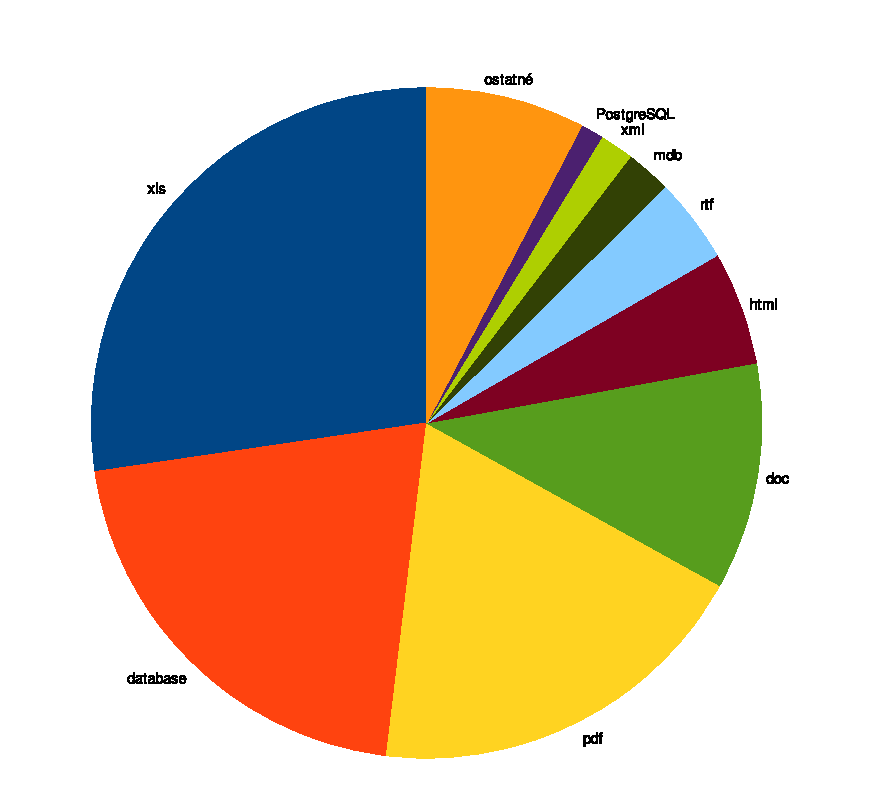
\includegraphics[width=9cm]{dataset_formaty}
\caption{Zastúpenie jednotlivých formátov medzi zverejniteľnými datasetmi, s ktorých zverejnením rezorty súhlasili.}
\label{formaty}
\end{figure}

Ďalej ukážeme, ako je na tom zverejňovanie datasetov pre jednotlivých prevádzkovateľov. Obrázok \ref{zverejnene} ukazuje, aká časť zverejniteľných datasetov, s ktorých zverejnením rezort súhlasil, je zverejnená na data.gov.sk. Dá sa vidieť, že väčšina prevádzkovateľov súhlasila so zverejnením viacerých datasetov ako je naozaj zverejnených.

\begin{figure}
\center 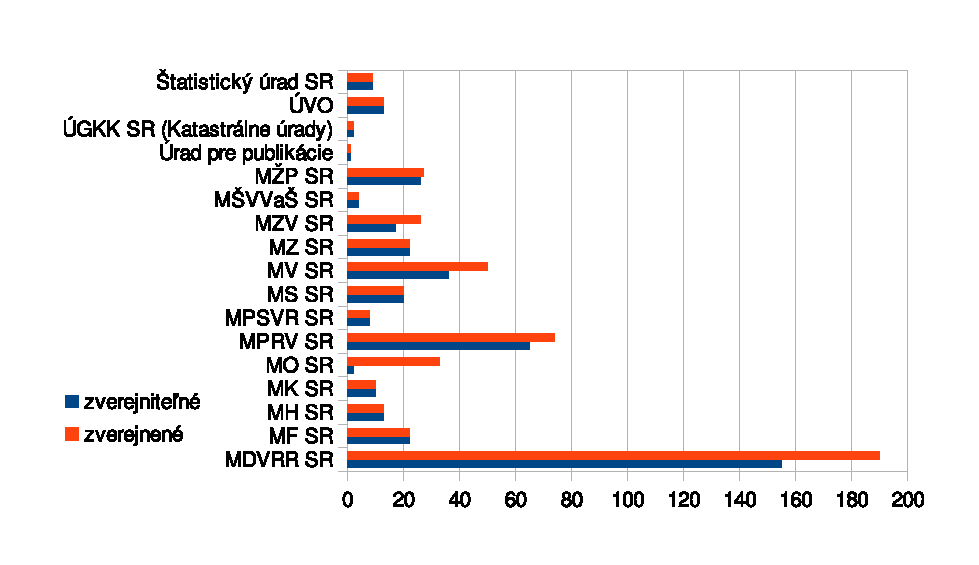
\includegraphics[width=14cm]{zverejnene_prevadzkovatel}
\caption{Zverejené a zverejniteľné datasety pre jednotlivých prevádzkovateľov.}
\label{zverejnene}
\end{figure}

Pri hľadaní dôvodu sme sa pozreli na formáty zverejniteľných, ale ešte nezverejnených datasetov. Obrázok \ref{nezverejnene_formaty} ukazuje distribúciu jednotlivých formátov. Dá sa vidieť, že medzi nezvernenými datasetmi je najviac datasetov vo formáte databázy. Predpokladáme, že export dát z databázy v otvorenom formáte často nie je taký jednoduchý.

\begin{figure}
\center 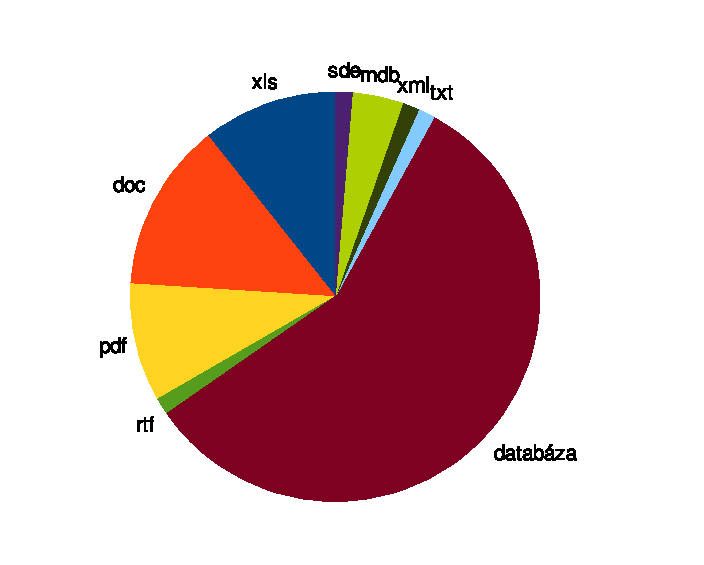
\includegraphics[width=14cm]{nezverejnene_formaty}
\caption{Zastúpenie formátov medzi nezverejnenými, ale zverejniteľnými datasetmi.}
\label{nezverejnene_formaty}
\end{figure}

Na koniec sa pozrieme na stav datasetov zverejnených na data.gov.sk. Obrázok \ref{stars} ukazuje hodnotenie datasetov podľa 5 hviezdičkového hodnotenia z \ref{5star}. Vidíme, že väčšina datasetov má 3 hviezdičky. To značí datasety, ktoré majú otvorený formát a sú štrukturované. Treba ale myslieť na to, že v skutočnosti nemá väčšina datasetov ani jednu hviezdičku, lebo nemajú otvorenú licenciu.

Tiež sa pozrieme na dostupnosť jednotlivých datasetov. Obrázok \ref{status} ukazuje, aký je stav datasetov na data.gov.sk. Vidíme, že väčšina datasetov je v poriadku dostupná. Ale niekoľko datasetov nie je dostupných. Tak isto existujú na data.gov.sk datasety, ktorých zdroj presmeruje na inú stránku. Tak isto je na obrázku \ref{status} ukázané, koľko datasetov je prístupných iba po vyplnení webového formulára.

\begin{figure}
\center 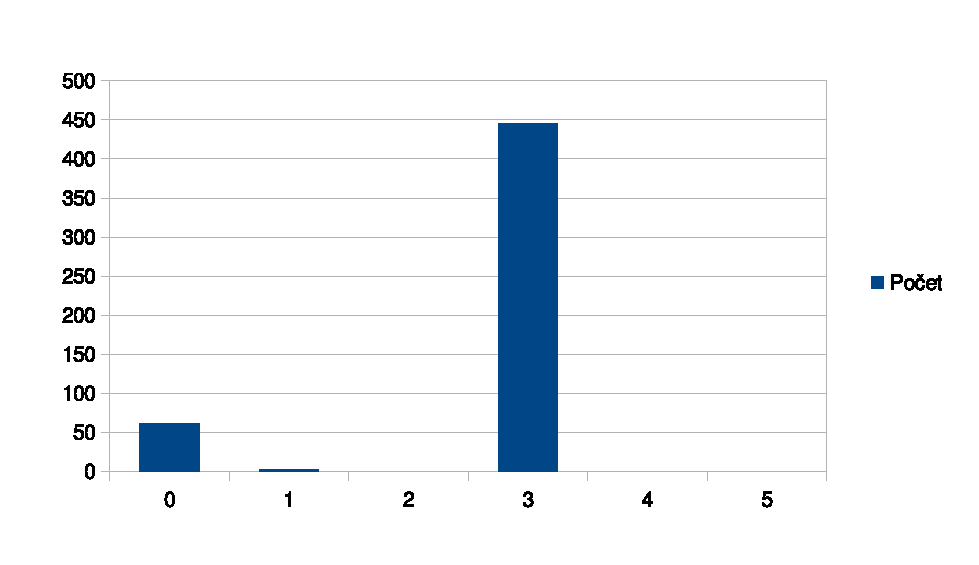
\includegraphics[width=14cm]{stars}
\caption{Počty datasetov pre jednotlivé hodnotenia.}
\label{stars}
\end{figure}

\begin{figure}
\center 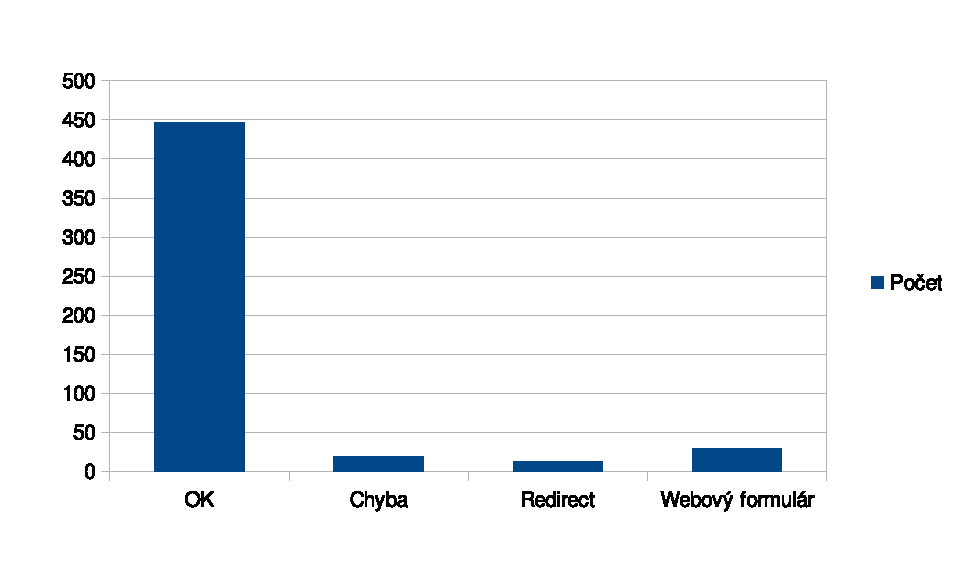
\includegraphics[width=14cm]{status}
\caption{Počty datasetov v jednotlivých stavoch.}
\label{status}
\end{figure}

TODO - počkať na Maťa 



  - čo ste riešili? (vstup, výstup)
TODO - Edo, Johnny 

VSTUP: zoznam datasetov na data.gov.sk
VYSTUP: pre každý dataset, prejsť všetky linky, zistiť, či žijú a či odkazujú na nejaký súbor.
      Ak neodkazujú na súbor, zistil, či bol redirect, ak nebol je to pravdepodobne webový formulár. 
      Ak je výstup súbor, pozrieť content disposition, príponu v prehliadači a content-type. Uhádnuť príponu súboru a na základe 
       jednoduchej heuristiky prideliť počet hviezdičiek podľa http://5stardata.info/

  - HLAVNE: aké sú výsledky? (štatistiky, tabuľka, graf) 

pokiaľ si správne spomínam Maťo slúbil to spracovať do štatistík. 
Aktuálny dump databázy pushnem čoskoro, keď dobehne skript.


  - čo bolo najťažšie? 
  - 1-3 zaujímavostí (kľudne hate, ... aby to oživilo prezentáciu :P)

srali ma akurát tie dva datasety na ktorých to padalo a nevedel som zistiť prečo.


%\subsection{Vyhľadávanie ďalších datasetov}
%TODO zopar sample queries na vsetky, resp. konkretne z 525

\section{Záver} 

TODO - na koniec 

\paragraph{Budúca práca} 

Zobrať názvy z \ref{525} a vyhľadať chýbajúce datasety na slovenskom Internete. 

Vygenerovať zoznam štátnych inštitúcií a automaticky vyhľadávať potenciálne datasety.

Obe boli nad rámec rozsahu našej práce. 

\section{Referencie} 
\begin{itemize} 
  \item \label{proj} \href{https://github.com/koniiiik/opendata-sk-ias}{Repozitár násho projektu s dokumentáciou}. %TODO - ensure only zverejnitelne
  \item \label{525} \href{http://www.otvorenavlada.gov.sk/datasety-statnej-spravy/}{Zoznam datasetov \emph{užitočných} na zverejnenie}.
  \item \label{hodnotenie} \href{http://www.otvorenavlada.gov.sk/navrh-hodnotiacej-spravy-iniciativy-pre-otvorene-vladnutie-v-slovenskej-republike/}{Návrh hodnotiacej správy Iniciatívy pre otvorené vládnutie v Slovenskej republike}.
  \item \label{kvalita} \href{http://www.zbierka.sk/sk/predpisy/55-2014-z-z.p-35621.pdf}{Výnos 55/2014} aj o kvalite OpenData. 
  \item \label{hany} \href{https://github.com/hanecak/data.gov.sk-link-check/}{Link check} datasetov portálu. 
\end{itemize} 


\section{Príloha - Vysvetlenie pojmov}
\subsection{OpenData} 
\label{opendata} 
TODO prelozit 
Open data is the idea that certain data should be freely available to everyone to use and republish as they wish, without restrictions from copyright, patents or other mechanisms of control.[1] The goals of the open data movement are similar to those of other "Open" movements such as open source, open hardware, open content, and open access. The philosophy behind open data has been long established (for example in the Mertonian tradition of science), but the term "open data" itself is recent, gaining popularity with the rise of the Internet and World Wide Web and, especially, with the launch of open-data government initiatives such as Data.gov and Data.gov.uk.


\subsection{Hodnotenie kvality datasetov}
\label{zakon-kvalita} 
Podľa \href{http://www.zbierka.sk/sk/predpisy/55-2014-z-z.p-35621.pdf}{výnosu 55/2014} popisujúci aj kvalitu OpenData. 

Kvalita datasetu poskytovaného povinnou osobou
(1) Štandardom kvality datasetu poskytovaného po-
vinnou osobou je rozdelenie kvality datasetu na šesť
úrovní, ktorými sú
a) úroveň 0, pri ktorej nie je dataset poskytovaný
v elektronickej forme,
b) úroveň 1, pri ktorej je dataset dostupný vo webovom
prostredí,
c) úroveň 2, pri ktorej je splnená požiadavka uvedená
v písmene b) a obsah datasetu je štruktúrovaný tak,
že umožňuje automatizované spracovanie,
d) úroveň 3, pri ktorej sú splnené požiadavky uvedené
v písmene c) a dataset je poskytovaný v otvorenom
formáte, nezávislom na konkrétnom proprietárnom
softvéri,
e) úroveň 4, pri ktorej sú splnené požiadavky uvedené
v písmene d) a na identifikáciu údajov datasetu a ich
vzťahov sa používajú refencovateľné identifikátory,
f) úroveň 5, pri ktorej sú splnené požiadavky uvedené
v písmene e) a dataset a jeho interné a externé
vzťahy majú charakter identifikátormi prepojených
údajov.
(2) Ak sa údaje poskytujú pre automatizované spra-
covanie, štandardom kvality datasetu poskytovaného
povinnou osobou je aj ich poskytovanie ako datasetu
s otvorenými údajmi podľa § 53 a v kvalite najmenej
úrovne 3.

CKAN plugin 
https://github.com/ckan/ckanext-qa


\end{document} 
